\documentclass[../main.tex]{subfiles}
\begin{document}
\section{概念学习}\label{sec:concept-learning}

\subsection{归纳学习简介}
\begin{enumerate}
 \item \textbf{归纳学习}
    \begin{itemize}
        \item \textbf{归纳学习：}从特殊的样例得到普遍的规律（从特殊到一般）
        \item \textbf{归纳：}只能保证输出的假设能与训练样例相拟合
        \item \textbf{归纳假设的一个基本假定：}对于未见实例最好的假设就是与训练数据最佳拟合的假设。
        \item \textbf{归纳学习假设：}任一假设如果在足够大的训练样例集中很好地逼近目标函数，它也能在未见实例中很好地逼近目标函数。
    \end{itemize}
\end{enumerate}

\subsection{概念学习简介}
\begin{enumerate}
    \item \textbf{概念学习}\footnote{概念学习是归纳学习里一个非常基础、非常典型的形式。}
    \begin{itemize}
        \item \textbf{概念学习：}给定某一类别的若干正例和反例，从中获得该类别的一般定义\footnote{概念学习就是指从有关某个布尔函数的输入输出训练样例中推断出该布尔函数。}。
        \item \textbf{概念：}可被看作一个对象或事件集合，它是从更大的集合中选取的子集，或在这个较大集合中定义的布尔函数。
        \item \textbf{概念学习问题：}给定一个样例集合以及每个样例是否属于某个概念的标注，怎样推断出该概念的一般定义。又称从样例中逼近布尔函数。
        \small\kaishu{
        例子：
        \begin{itemize}
            \item 目标概念：Aldo进行水上运动的日子，表示为布尔函数EnjoySport
            \item 任务目的：基于某天的各属性，预测EnjoySport的值
            \item 给定一个样例集D：每个样例表示为6个属性的集合
        \end{itemize}
        }
        \begin{figure}[H]
            \centering
            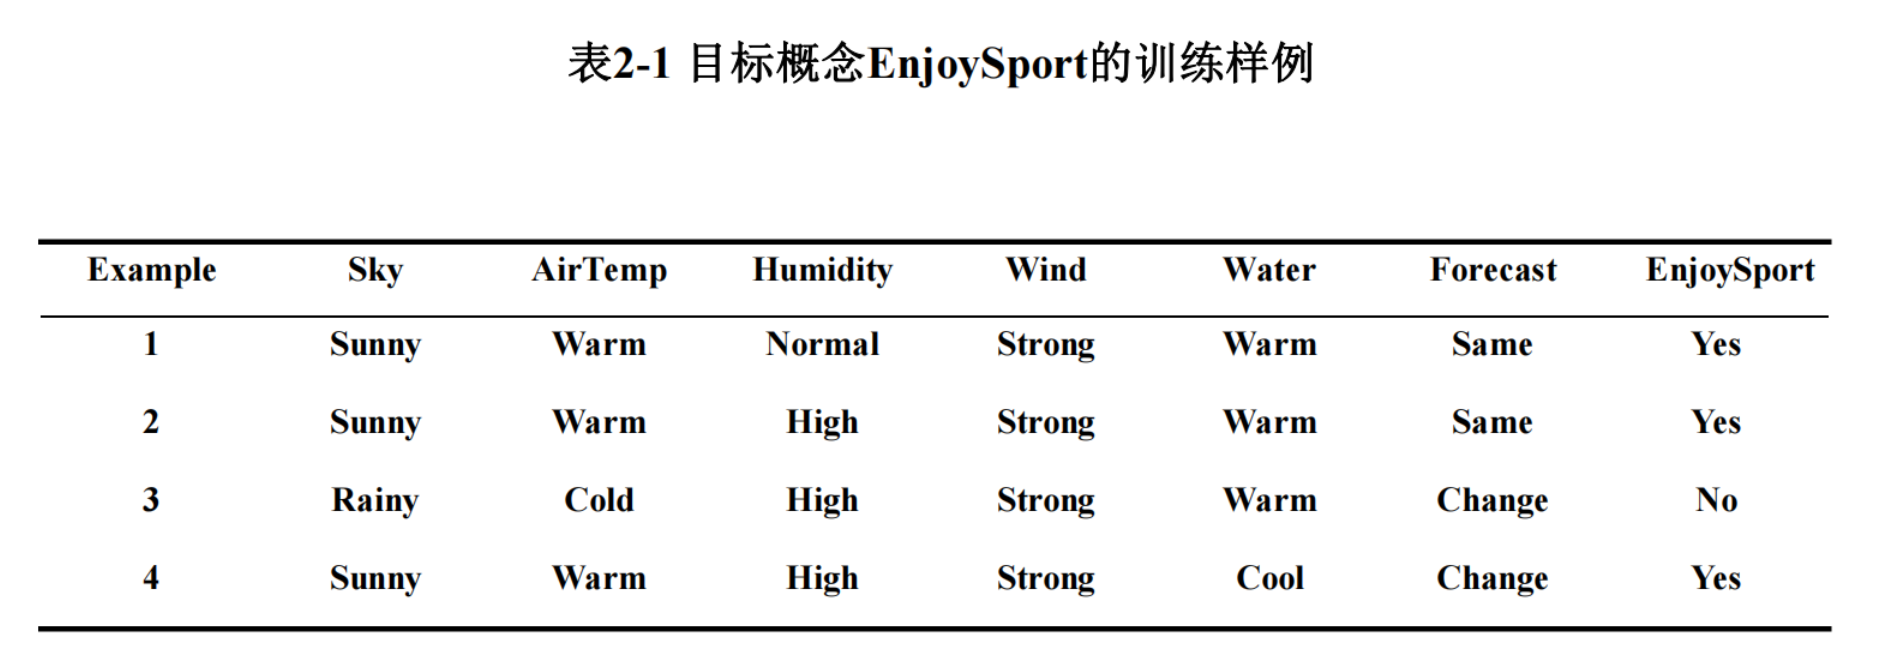
\includegraphics[width=1.0\linewidth]{images/enjoysport.png}
            \caption{目标概念enjoysport的训练样例}
            \label{fig:placeholder}
        \end{figure}
    \end{itemize}
        \item \textbf{假设的表示形式}
        \begin{itemize}
            \item \textbf{目标函数的表示：}一个简单的表示形式是实例各属性约束的合取式\footnote{在 EnjoySport 例子中，每个假设可表示为 6 个约束（或变量）组成的向量，每个约束对应一个属性的取值范围。}。
            \item 每个属性上的约束可以写成以下三种形式：
            \begin{itemize}
                \item \textbf{?}：表示该属性可接受任意值；
                \item 某个明确指定的属性值：表示该属性只能取该值；
                \item \textbf{$\phi$}：表示该属性不接受任何值。
            \end{itemize}
            \item \small\kaishu{
            例子：
            \begin{itemize}
                \item $\langle ?, \text{Cold}, \text{High}, ?, ?, ? \rangle$
                \item $\langle ?, ?, ?, ?, ?, ? \rangle$：所有样例都是正例
                \item $\langle \phi, \phi, \phi, \phi, \phi, \phi \rangle$：所有样例都是反例
            \end{itemize}
            }
        \end{itemize}

        \item \textbf{概念学习任务的形式化描述}\footnote{说人话就是，对每个属性，要么指定一个具体值，要么写 $?$ 表示无所谓，要么写 $\phi$ 表示不可能。然后机器学习的目标，就是从这些可能的规则里，找到一个能正确区分正例和反例的规则。例如在 EnjoySport 任务中，学习器根据若干天的天气属性及其“是否适合进行水上运动”的标记，归纳出一个判定规则，如 $\langle \text{Sunny}, \text{Warm}, ?, ?, ?, ? \rangle$，表示当天空为 Sunny 且气温为 Warm 时，预测该日属于目标概念。}
        \begin{itemize}
            \item \textbf{已知：}
            \begin{itemize}
                \item \textbf{实例集 $X$：}每个实例 $x$ 由 6 个属性描述，每个属性的取值范围已确定。
                \item \textbf{假设集 $H$：}每个假设 $h$ 描述为 6 个属性取值约束的合取。
                \item \textbf{目标概念 $c$：}一个布尔函数，变量为实例。
                \[
                c : X \rightarrow \{0,1\}
                \]
                \item \textbf{训练样例集 $D$：}由目标概念的正例和反例构成。
            \end{itemize}
            \item \textbf{求解目标：}在 $H$ 中寻找一个假设 $h$，使得对于 $X$ 中任意实例 $x$，都有
            \[
                h(x) = c(x)
            \]
        \end{itemize}
    \item \textbf{概念学习可看作搜索过程}\footnote{一旦选定假设的表示形式，实际上就确定了一个\textbf{假设空间}，学习的过程就是在这个空间中搜索合适的假设。}
    \begin{itemize}
        \item \textbf{搜索范围：}由假设表示形式所隐含定义的整个假设空间。
        \item \textbf{搜索目标：}找到能够尽可能拟合训练样例的假设。
    \end{itemize}
    {\small\kaishu
    例题：EnjoySport 例子的空间大小\label{enjoy_sport}
    \begin{itemize}
        \item 设属性 \textit{Sky} 有 3 种可能取值，属性 \textit{AirTemp}、\textit{Humidity}、\textit{Wind}、\textit{Water} 和 \textit{Forecast} 各有 2 种可能取值。
        \item 则实例空间 $X$ 的大小为
        \[
            |X| = 3 \times 2 \times 2 \times 2 \times 2 \times 2 = 96
        \]
        即共有 96 种不同实例。
        \item 对于假设空间 $H$，每个属性的约束可以取“具体属性值”“?” 或 “$\phi$”。
        \item 因此语法形式上共有
        \[
            |H| = 5 \times 4 \times 4 \times 4 \times 4 \times 4 = 5120
        \]
        种假设。
        \item 但从语义上看，只要假设中某一位出现 $\phi$，该假设就不会接受任何实例，因此所有包含 $\phi$ 的假设在语义上等价于“把所有实例都判为反例”。
        \item 所以语义不同的假设总数为
        \[
            1 + 4 \times 3 \times 3 \times 3 \times 3 \times 3 = 973
        \]
        其中前面的 $1$ 表示“所有实例都判为反例”的那一类假设。
    \end{itemize}    
    }
    
    \item \textbf{假设的一般到特殊序关系}
    
    {\small\kaishu
    例如，考虑下面两个假设：
        \[
            h_1 = \langle \text{Sunny}, ?, ?, \text{Strong}, ?, ? \rangle
        \]
        \[
            h_2 = \langle \text{Sunny}, ?, ?, ?, ?, ? \rangle
        \]
    
    任何被 $h_1$ 判为正例的实例一定也会被 $h_2$ 判为正例，因此 $h_2$ 比 $h_1$ 更一般\footnote{利用这种“一般到特殊”的关系，可以不必枚举全部假设，而是在假设空间中更有效地搜索。}
    }
    \item \textbf{关系定义}：
    \begin{itemize}
         \item \textbf{“满足”：}对任意实例 $x$ 和假设 $h$，若 $h(x)=1$，则称实例 $x$ \textbf{满足}假设 $h$ \footnote{$x$被$h$划定的范围包括了}。
        \item \textbf{“更一般”：}设 $h_j$ 和 $h_k$ 是定义在实例空间 $X$ 上的布尔函数，若对任意 $x \in X$，只要 $h_k(x)=1$ 就必有 $h_j(x)=1$，即：
            \[
                (\forall x \in X)\bigl[(h_k(x)=1)\rightarrow(h_j(x)=1)\bigr]
            \]
            则称 $h_j$ 比 $h_k$ 更一般，记为
            \[
                h_j \geq_g h_k
            \]
        \item \textbf{“严格更一般”}：若
            \[
                h_j \geq_g h_k \quad \text{且} \quad h_k \not\geq_g h_j
            \]
            则称 $h_j$ 严格比 $h_k$ 更一般，记为
            \[
                h_j >_g h_k
            \]
        \item \textbf{“更特殊”}：若
            \[
                h_k \geq_g h_j
            \]
            则称 $h_j$ 比 $h_k$ 更特殊，记为
            \[
                h_j \leq_g h_k
            \]
    \end{itemize}
    \item \textbf{偏序\footnote{偏序即有些能比较，有些不能比较，比无序有结构，但不像全序那么整齐；无序即元素之间几乎没关系，只能一个个看；全序即任意两个元素都能比较大小，像排好序的数组。}的特点：}全序上的搜索可以是二分法，偏序的搜索比无序简单，比全序复杂。偏序关系的定义与目标概念无关\footnote{更一般或者更特殊只与假设本身覆盖的范围决定，和真实答案$c$是什么没啥关系。}。

\end{enumerate}

\subsection{Find-S：寻找极大特殊假设}\label{sec:find-s}
\begin{enumerate}
    \item \textbf{Find-S 算法的基本思想：}Find-S 是一种利用 more\_general\_than 偏序\footnote{从特殊到一般}在假设空间中进行搜索的算法\footnote{其搜索策略是：从假设空间 $H$ 中最特殊的假设开始，当当前假设不能覆盖正例时，再将其作最小必要的一般化。}

    \item \textbf{Find-S 算法步骤}
    \begin{enumerate}
        \item 将 $h$ 初始化为 $H$ 中最特殊的假设：
        \[
            h \leftarrow \langle \phi,\phi,\phi,\phi,\phi,\phi \rangle
        \]
        \item 对每个正例 $x$，依次检查 $h$ 的每个属性约束 $a_i$：
        \begin{itemize}
            \item 若 $x$ 满足 $a_i$，则该属性约束保持不变；
            \item 若 $x$ 不满足 $a_i$，则将 $a_i$ 替换为能够使 $x$ 被满足的、比当前约束更一般的最小约束。
        \end{itemize}
        \item 输出最终假设 $h$。
    \end{enumerate}

    \item \textbf{Find-S 在 EnjoySport 上的应用}
    \begin{figure}[H]
        \centering
        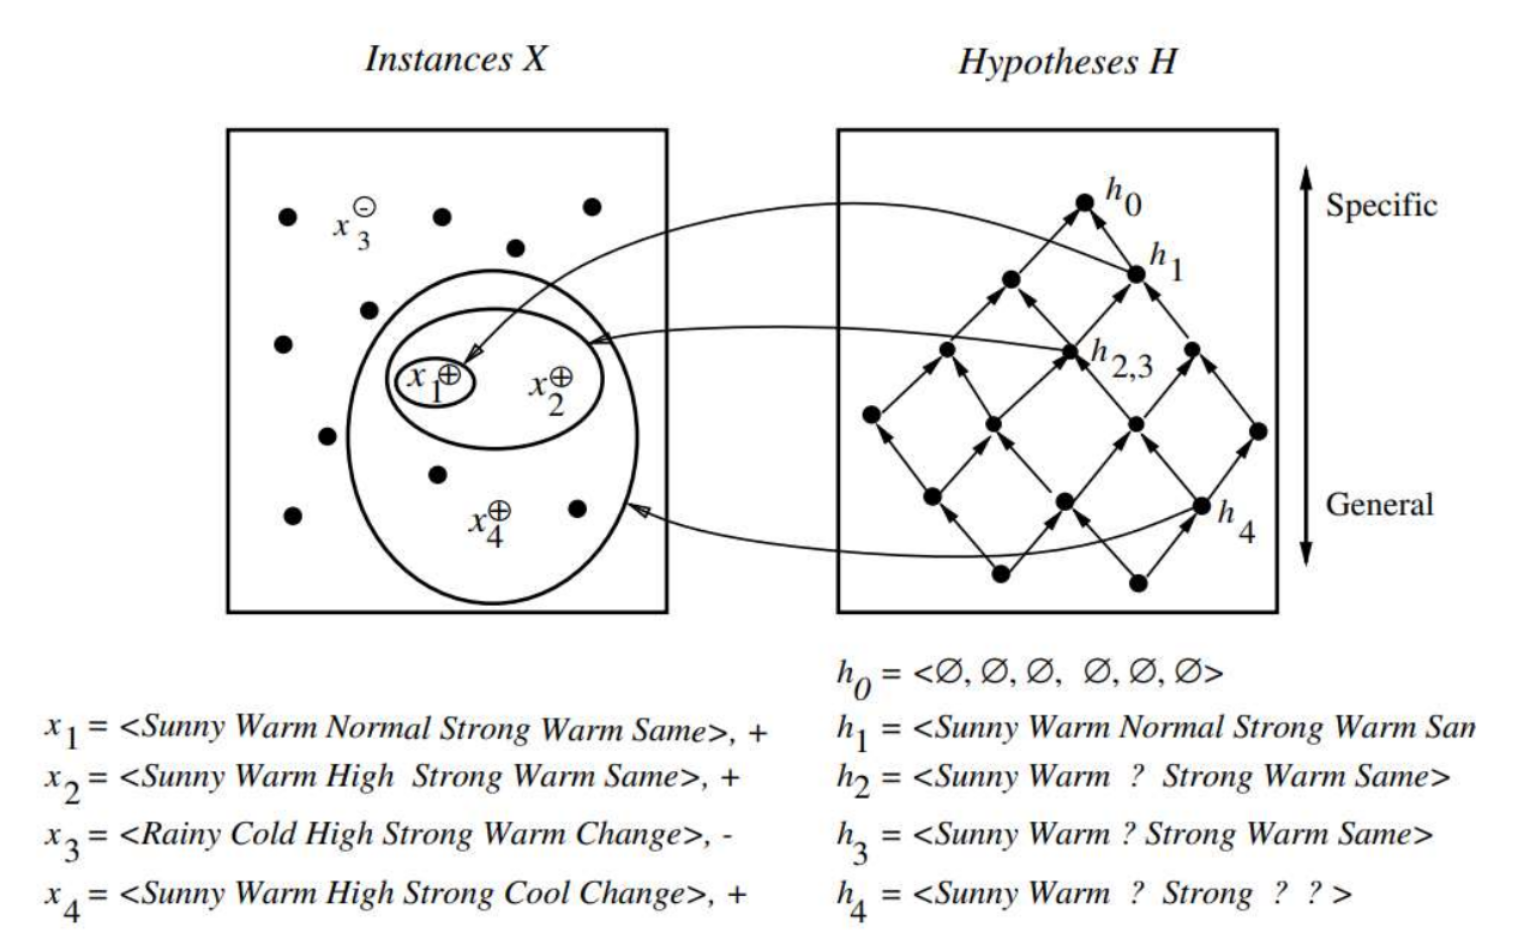
\includegraphics[width=1\linewidth]{images/finds_enjoy.png}
        \caption{Find-S 在 EnjoySport 上的应用}
        \label{fig:placeholder}
    \end{figure}
    {\small\kaishu
    \begin{itemize}
        \item 初始时取最特殊假设：
        \[
            h \leftarrow \langle \phi,\phi,\phi,\phi,\phi,\phi \rangle
        \]
        \item 观察到第一个训练样例为正例时，当前假设过于特殊，因此每个属性都替换为该正例对应的属性值：
        \[
            h \leftarrow \langle \text{Sunny},\text{Warm},\text{Normal},\text{Strong},\text{Warm},\text{Same} \rangle
        \]
        \item 再观察到第二个训练样例仍为正例时，将当前假设中与该正例不一致的属性作最小一般化，于是得到：
        \[
            h \leftarrow \langle \text{Sunny},\text{Warm}, ?, \text{Strong},\text{Warm},\text{Same} \rangle
        \]
        \item 之后若遇到反例，Find-S 不修改当前假设。
        \item 随着新的正例继续加入，假设继续按最小必要原则一般化，例如可进一步得到：
        \[
            h \leftarrow \langle \text{Sunny},\text{Warm}, ?, \text{Strong}, ?, ? \rangle
        \]
    \end{itemize}
    }
    
    \item \textbf{Find-S 的重要特点}：对于由属性约束合取式构成的假设空间 $H$，Find-S 输出的是 $H$ 中与所有正例一致的极大特殊假设。

    \item \textbf{Find-S 的局限性}：输出的假设只是H中能够拟合训练样例的多个假设中的一个。
    {\small\kaishu
    \begin{itemize}
        \item 算法只利用正例更新假设，未显式利用反例信息。
        \item 它不能判断最终假设是否已经收敛到真实目标概念。
        \item 它默认训练样例彼此一致，若数据存在噪声或标注冲突，算法可能失效。
        \item 若假设空间中存在多个与正例一致的极大特殊假设，Find-S 不能完整表示这种不确定性。
    \end{itemize}
    }
\end{enumerate}


\subsection{变型空间和候选消除算法}\label{sec:candidate-elimination}
\begin{enumerate}
    \item \textbf{候选消除算法概述}
    \begin{itemize}
        \item \textbf{候选消除算法（candidate-elimination）：}输出与训练样例一致的所有假设的集合\footnote{候选消除算法在描述这一集合时不需要明确列举所有成员。}。
        \item 候选消除算法利用 more\_general\_than 偏序结构，可以维护一个一致假设集合的简洁表示。
        \item \textbf{缺点:}容错性较差。
    \end{itemize}

    \item \textbf{一致与变型空间}
    \begin{itemize}
        \item \textbf{一致（consistent）\footnote{这里的“一致”与前面定义的“满足”不同；“满足”只表示 $h(x)=1$，而“一致”要求 $h(x)$ 与真实标记 $c(x)$ 相同。“满足”针对的是$x$和$h$的关系，不论$x$是目标概念的正例还是反例。“一致”与目标概念有关，针对的是$h$和$c$的关系}：}若假设 $h$ 对训练样例集 $D$ 中每个样例 $\langle x, c(x) \rangle$ 都满足
        \[
            h(x) = c(x)
        \]
        则称 $h$ 与 $D$ 一致，记为
        \[
            \mathrm{Consistent}(h,D) \iff (\forall \langle x,c(x)\rangle \in D)\, h(x)=c(x)
        \]
        \textcolor{red}{理解：样本是真正例，h 也判成正例；样本是真反例，h 也判成反例}
        \item \textbf{变型空间（Version Space）：}与训练样例 $D$ 一致的所有假设组成的集合，包含了目标概念的所有合理的变型。
        \item 关于假设空间 $H$ 和训练样例集 $D$ 的变型空间记为下式，是$H$中与训练样例$D$一致的所有假设构成的子集
        \[
            VS_{H,D}=\{\,h\in H \mid \mathrm{Consistent}(h,D)\,\}
        \]
    \end{itemize}

    \item \textbf{列表后消除算法}\footnote{一种直接表示变型空间的方法是显式列出其所有成员。该方法能够得到与训练数据一致的全部假设，但要求显式枚举假设空间 $H$ 的所有成员，因此仅在 $H$ 有限且规模较小时才可行。}
    \begin{itemize}
        \item 算法过程如下：
        \begin{enumerate}
            \item 将变型空间初始化为包含 $H$ 中所有假设的集合；
            \item 对每个训练样例 $\langle x,c(x)\rangle$，从当前集合中删除所有满足
            $
                h(x)\neq c(x)
            $
            的假设；
            \item 输出剩余假设构成的集合。
        \end{enumerate}
    \end{itemize}

    \item \textbf{候选消除算法}\footnote{候选消除算法与列表后消除算法遵循相同原则，但不再显式列举全部一致假设。}
    \begin{itemize}
        \item 它仅用变型空间中两类边界成员来表示整个变型空间：
        \begin{itemize}
            \item \textbf{一般边界 $G$：}与 $D$ 一致的极大一般假设集合；
            \[
            G=\{\,g\in H \mid \mathrm{Consistent}(g,D)\land \neg \exists g' \in H \bigl[(g' >_g g)\land \mathrm{Consistent}(g',D)\bigr]\,\}
            \]
            \item \textbf{特殊边界 $S$：}与 $D$ 一致的极大特殊假设集合。
            \[
            S=\{\,s\in H \mid \mathrm{Consistent}(s,D)\land \neg \exists s' \in H \bigl[(s >_g s')\land \mathrm{Consistent}(s',D)\bigr]\,\}
            \]
        \end{itemize}
    \end{itemize}
    \begin{figure}[H]
        \centering
        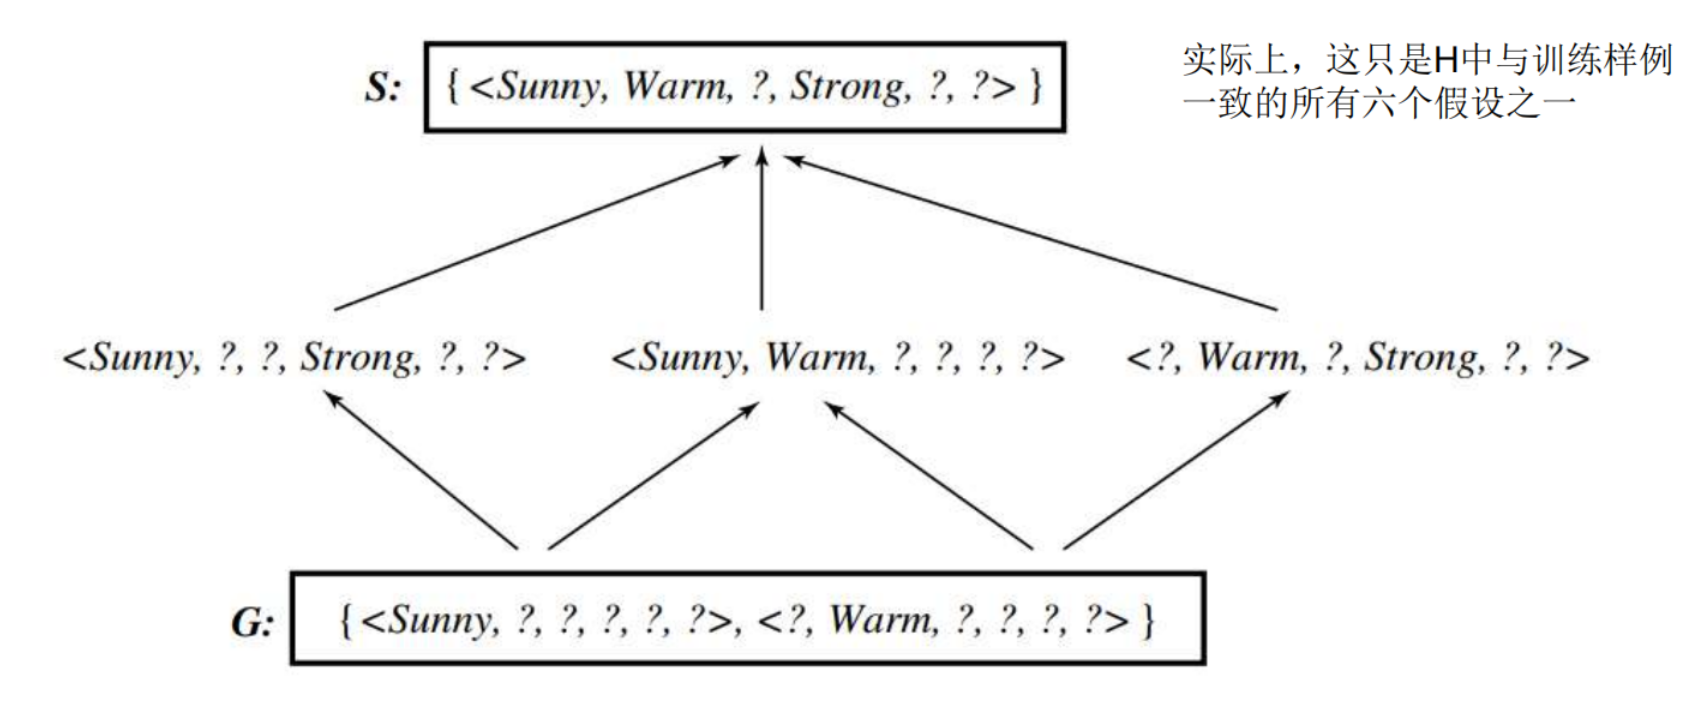
\includegraphics[width=1\linewidth]{images/GandS.png}
        \caption{变型空间的更简洁表示示例}
        \label{fig:placeholder}
    \end{figure}

    \item \textbf{变型空间表示定理}\footnote{人话：一个假设属于变型空间，当且仅当它位于某个一般边界成员与某个特殊边界成员之间。}
    \begin{itemize}
        \item 对任意实例集 $X$、定义在 $X$ 上的布尔假设空间 $H$、目标概念 $c:X\to\{0,1\}$ 以及训练样例集 $D=\{\langle x,c(x)\rangle\}$，若 $S$ 与 $G$ 定义良好，则有
        \[
            VS_{H,D}=
            \{\,h\in H \mid (\exists s\in S)(\exists g\in G)(g \geq_g h \geq_g s)\,\}
        \]
    \end{itemize}

    \item \textbf{候选消除算法流程}
    \begin{itemize}
        \item \textbf{初始化：}
        \[
            G \leftarrow \{\langle ?, ?, ?, ?, ?, ? \rangle\},\qquad
            S \leftarrow \{\langle \phi,\phi,\phi,\phi,\phi,\phi \rangle\}
        \]
        \item 对每个训练样例 $d$：
        \begin{itemize}
            \item 若 $d$ 为正例：
            \begin{itemize}
                \item 从 $G$ 中删除所有与 $d$ 不一致的假设；
                \item 对 $S$ 中每个与 $d$ 不一致的假设 $s$，将其从 $S$ 中删除，并加入 $s$ 的所有\textbf{极小一般化式} $h$，其中 $h$ 与 $d$ 一致，且存在某个 $g\in G$ 使得
                \[
                    g \geq_g h
                \]
                \item 从 $S$ 中删除所有比集合中其他成员更一般的假设\footnote{实际上就是去重的意思，一般在上面的极小一般化式的过程中直接隐式地做掉了，不懂的话可以看一下下面的例子}。
            \end{itemize}
            \item 若 $d$ 为反例：
            \begin{itemize}
                \item 从 $S$ 中删除所有与 $d$ 不一致的假设；
                \item 对 $G$ 中每个与 $d$ 不一致的假设 $g$，将其从 $G$ 中删除，并加入 $g$ 的所有\textbf{极小特殊化式} $h$，其中 $h$ 与 $d$ 一致，且存在某个 $s\in S$ 使得
                \[
                    h \geq_g s
                \]
                \item 从 $G$ 中删除所有比集合中其他成员更特殊的假设。
            \end{itemize}
        \end{itemize}
        \item 算法结束时，由边界集合 $S$ 和 $G$ 共同给出当前训练数据对应的变型空间。
    \end{itemize}
\textcolor{red}{来一个正例：删除 $G$ 中不能把该正例判为真的假设；删除 $S$ 中不能把该正例判为真的假设，并加入这些被删除假设的极小一般化形式（要求$G$中存在假设比该极小一般化形式还一般），最后删除 $S$ 中比其他成员更一般的假设；}

\textcolor{blue}{来一个反例：删除 $S$ 中不能把该反例判为假的假设；删除 $G$ 中不能把该反例判为假的假设，并加入这些被删除假设的极小特殊化形式（要求$S$中存在假设比该极小特殊化形式还特殊），最后删除 $G$ 中比其他成员更特殊的假设\\}
    \item \textbf{候选消除算法示例（EnjoySport）}

	\textbf{例题1：}

    {\small\kaishu
    \begin{itemize}
        \item 考虑下面 4 个训练样例：
        \[
        \begin{aligned}
            x_1 &= \langle \text{Sunny}, \text{Warm}, \text{Normal}, \text{Strong}, \text{Warm}, \text{Same} \rangle, + \\
            x_2 &= \langle \text{Sunny}, \text{Warm}, \text{High}, \text{Strong}, \text{Warm}, \text{Same} \rangle, + \\
            x_3 &= \langle \text{Rainy}, \text{Cold}, \text{High}, \text{Strong}, \text{Warm}, \text{Change} \rangle, - \\
            x_4 &= \langle \text{Sunny}, \text{Warm}, \text{High}, \text{Strong}, \text{Cool}, \text{Change} \rangle, +
        \end{aligned}
        \]

        \item \textbf{初始化：}
        \[
            S_0=\{\langle \phi,\phi,\phi,\phi,\phi,\phi \rangle\},\qquad
            G_0=\{\langle ?, ?, ?, ?, ?, ? \rangle\}
        \]

        \item \textbf{处理正例 $x_1$：}
        \begin{itemize}
            \item 先删除 $G_0$ 中不能把该正例判为真的假设。由于
            \[
                \langle ?, ?, ?, ?, ?, ? \rangle
            \]
            能把任意样本判为正，因此与正例 $x_1$ 一致，故 $G$ 不变。
            \item 再删除 $S_0$ 中不能把该正例判为真的假设。当前唯一成员
            \[
                \langle \phi,\phi,\phi,\phi,\phi,\phi \rangle
            \]
            会把任意样本都判为负，因此不能把 $x_1$ 判为真，需要删除。
            \item 对被删除假设加入其极小一般化形式。由于 $x_1$ 是第一个正例，因此其极小一般化形式就是
            \[
                \langle \text{Sunny}, \text{Warm}, \text{Normal}, \text{Strong}, \text{Warm}, \text{Same} \rangle
            \]
            且 $G_0$ 中存在更一般的假设
            \[
                \langle ?, ?, ?, ?, ?, ? \rangle
            \]
            满足
            \[
                g \geq_g h
            \]
            因此保留该一般化结果。
            \item 最后删除 $S$ 中比其他成员更一般的假设。此时 $S$ 中只有一个成员，无需删除。
            \item 更新后
            \[
                S_1=\{\langle \text{Sunny}, \text{Warm}, \text{Normal}, \text{Strong}, \text{Warm}, \text{Same} \rangle\}
            \]
            \[
                G_1=\{\langle ?, ?, ?, ?, ?, ? \rangle\}
            \]
        \end{itemize}

        \item \textbf{处理正例 $x_2$：}
        \begin{itemize}
            \item 先删除 $G_1$ 中不能把该正例判为真的假设。由于
            \[
                \langle ?, ?, ?, ?, ?, ? \rangle
            \]
            仍能把 $x_2$ 判为真，因此 $G$ 不变。
            \item 再删除 $S_1$ 中不能把该正例判为真的假设。当前
            \[
                \langle \text{Sunny}, \text{Warm}, \text{Normal}, \text{Strong}, \text{Warm}, \text{Same} \rangle
            \]
            在 Humidity 上与 $x_2$ 不一致，因此不能把 $x_2$ 判为真，需要删除。
            \item 对被删除假设加入其极小一般化形式。为了恰好覆盖 $x_2$ 和 $x_1$，只需将第三个属性一般化为 $?$，得到
            \[
                \langle \text{Sunny}, \text{Warm}, ?, \text{Strong}, \text{Warm}, \text{Same} \rangle
            \]
            且 $G_1$ 中存在更一般的假设
            \[
                \langle ?, ?, ?, ?, ?, ? \rangle
            \]
            满足
            \[
                g \geq_g h
            \]
            因此保留。
            \item 最后删除 $S$ 中比其他成员更一般的假设。此时仍只有一个成员，无需删除。
            \item 更新后
            \[
                S_2=\{\langle \text{Sunny}, \text{Warm}, ?, \text{Strong}, \text{Warm}, \text{Same} \rangle\}
            \]
            \[
                G_2=\{\langle ?, ?, ?, ?, ?, ? \rangle\}
            \]
        \end{itemize}

        \item \textbf{处理反例 $x_3$：}
        \begin{itemize}
            \item 先删除 $S_2$ 中不能把该反例判为假的假设。当前
            \[
                \langle \text{Sunny}, \text{Warm}, ?, \text{Strong}, \text{Warm}, \text{Same} \rangle
            \]
            对 $x_3$ 的分类为负，因此能够把该反例判为假，故 $S$ 不变。
            \item 再删除 $G_2$ 中不能把该反例判为假的假设。当前
            \[
                \langle ?, ?, ?, ?, ?, ? \rangle
            \]
            会把所有样本都判为正，因此不能把反例 $x_3$ 判为假，需要删除。
            \item 对被删除假设加入其极小特殊化形式。为了排除 $x_3$ 并覆盖 $x_1$和$x_2$，同时仍保持比 $S_2$ 更一般，可保留的极小特殊化形式为
            \[
                \langle \text{Sunny}, ?, ?, ?, ?, ? \rangle,\qquad
                \langle ?, \text{Warm}, ?, ?, ?, ? \rangle,\qquad
                \langle ?, ?, ?, ?, ?, \text{Same} \rangle
            \]
            它们都满足存在某个 $s\in S_2$ 使得
            \[
                h \geq_g s
            \]
            因此保留。
            \item 最后删除 $G$ 中比其他成员更特殊的假设。上述 3 个假设彼此互不包含，因此都不是冗余成员，全部保留。
            \item 更新后
            \[
                S_3=\{\langle \text{Sunny}, \text{Warm}, ?, \text{Strong}, \text{Warm}, \text{Same} \rangle\}
            \]
            \[
                G_3=
                \left\{
                \langle \text{Sunny}, ?, ?, ?, ?, ? \rangle,\,
                \langle ?, \text{Warm}, ?, ?, ?, ? \rangle,\,
                \langle ?, ?, ?, ?, ?, \text{Same} \rangle
                \right\}
            \]
        \end{itemize}

        \item \textbf{处理正例 $x_4$：}
        \begin{itemize}
            \item 先删除 $G_3$ 中不能把该正例判为真的假设。由于
            \[
                \langle ?, ?, ?, ?, ?, \text{Same} \rangle
            \]
            不能覆盖 $x_4$，故将其删除；其余两个假设都能把 $x_4$ 判为真，因此保留。
            \item 再删除 $S_3$ 中不能把该正例判为真的假设。当前
            \[
                \langle \text{Sunny}, \text{Warm}, ?, \text{Strong}, \text{Warm}, \text{Same} \rangle
            \]
            在 Water 和 Forecast 两个属性上与 $x_4$ 不一致，因此不能把 $x_4$ 判为真，需要删除。
            \item 对被删除假设加入其极小一般化形式。为了恰好覆盖 $x_4$ 以及之前的$x_1\sim x_3$，只需将 Water 和 Forecast 两个属性一般化为 $?$，得到
            \[
                \langle \text{Sunny}, \text{Warm}, ?, \text{Strong}, ?, ? \rangle
            \]
            且此时 $G$ 中存在更一般的假设
            \[
                \langle \text{Sunny}, ?, ?, ?, ?, ? \rangle
            \]
            以及
            \[
                \langle ?, \text{Warm}, ?, ?, ?, ? \rangle
            \]
            满足
            \[
                g \geq_g h
            \]
            因此保留该极小一般化形式。
            \item 最后删除 $S$ 中比其他成员更一般的假设。此时只有一个成员，无需删除。
            \item 更新后
            \[
                S_4=\{\langle \text{Sunny}, \text{Warm}, ?, \text{Strong}, ?, ? \rangle\}
            \]
            \[
                G_4=
                \left\{
                \langle \text{Sunny}, ?, ?, ?, ?, ? \rangle,\,
                \langle ?, \text{Warm}, ?, ?, ?, ? \rangle
                \right\}
            \]
        \end{itemize}

        \item \textbf{最终结果：}
        \[
            S=\{\langle \text{Sunny}, \text{Warm}, ?, \text{Strong}, ?, ? \rangle\}
        \]
        \[
            G=
            \left\{
            \langle \text{Sunny}, ?, ?, ?, ?, ? \rangle,\,
            \langle ?, \text{Warm}, ?, ?, ?, ? \rangle
            \right\}
        \]
        因此，最终变型空间由所有满足
        \[
            (\exists s\in S)(\exists g\in G)(g \geq_g h \geq_g s)
        \]
        的假设 $h$ 构成。
    \end{itemize}
    }

\textbf{例题2：}\label{houxuan2}

{\small\kaishu
\begin{itemize}
    \item 考虑下面 4 个训练样例，并按逆序处理：
    \[
    \begin{aligned}
        x_4 &= \langle \text{Sunny}, \text{Warm}, \text{High}, \text{Strong}, \text{Cool}, \text{Change} \rangle, + \\
        x_3 &= \langle \text{Rainy}, \text{Cold}, \text{High}, \text{Strong}, \text{Warm}, \text{Change} \rangle, - \\
        x_2 &= \langle \text{Sunny}, \text{Warm}, \text{High}, \text{Strong}, \text{Warm}, \text{Same} \rangle, + \\
        x_1 &= \langle \text{Sunny}, \text{Warm}, \text{Normal}, \text{Strong}, \text{Warm}, \text{Same} \rangle, +
    \end{aligned}
    \]

    \item \textbf{初始化：}
    \[
        S_0=\{\langle \phi,\phi,\phi,\phi,\phi,\phi \rangle\},\qquad
        G_0=\{\langle ?, ?, ?, ?, ?, ? \rangle\}
    \]

    \item \textbf{处理正例 $x_4$：}
    \begin{itemize}
        \item 先删除 $G_0$ 中不能把该正例判为真的假设。由于
        \[
            \langle ?, ?, ?, ?, ?, ? \rangle
        \]
        能把任意样本判为正，因此与正例 $x_4$ 一致，故 $G$ 不变。
        \item 再删除 $S_0$ 中不能把该正例判为真的假设。当前唯一成员
        \[
            \langle \phi,\phi,\phi,\phi,\phi,\phi \rangle
        \]
        会把任意样本都判为负，因此不能把 $x_4$ 判为真，需要删除。
        \item 对被删除假设加入其极小一般化形式。由于 $x_4$ 是第一个正例，因此其极小一般化形式就是
        \[
            \langle \text{Sunny}, \text{Warm}, \text{High}, \text{Strong}, \text{Cool}, \text{Change} \rangle
        \]
        且 $G_0$ 中存在更一般的假设
        \[
            \langle ?, ?, ?, ?, ?, ? \rangle
        \]
        满足
        \[
            g \geq_g h
        \]
        因此保留该一般化结果。
        \item 最后删除 $S$ 中比其他成员更一般的假设。此时 $S$ 中只有一个成员，无需删除。
        \item 更新后
        \[
            S_1=\{\langle \text{Sunny}, \text{Warm}, \text{High}, \text{Strong}, \text{Cool}, \text{Change} \rangle\}
        \]
        \[
            G_1=\{\langle ?, ?, ?, ?, ?, ? \rangle\}
        \]
    \end{itemize}

    \item \textbf{处理反例 $x_3$：}
    \begin{itemize}
        \item 先删除 $S_1$ 中不能把该反例判为假的假设。当前
        \[
            \langle \text{Sunny}, \text{Warm}, \text{High}, \text{Strong}, \text{Cool}, \text{Change} \rangle
        \]
        对 $x_3$ 的分类为负，因此能够把该反例判为假，故 $S$ 不变。
        \item 再删除 $G_1$ 中不能把该反例判为假的假设。当前
        \[
            \langle ?, ?, ?, ?, ?, ? \rangle
        \]
        会把所有样本都判为正，因此不能把反例 $x_3$ 判为假，需要删除。
        \item 对被删除假设加入其极小特殊化形式。为了排除 $x_3$ 并保持比 $S_1$ 更一般，可保留的极小特殊化形式为
        \[
            \langle \text{Sunny}, ?, ?, ?, ?, ? \rangle,\qquad
            \langle ?, \text{Warm}, ?, ?, ?, ? \rangle,\qquad
            \langle ?, ?, ?, ?, \text{Cool}, ? \rangle
        \]
        它们都满足存在某个 $s\in S_1$ 使得
        \[
            h \geq_g s
        \]
        因此保留。
        \item 最后删除 $G$ 中比其他成员更特殊的假设。上述 3 个假设彼此互不包含，因此都不是冗余成员，全部保留。
        \item 更新后
        \[
            S_2=\{\langle \text{Sunny}, \text{Warm}, \text{High}, \text{Strong}, \text{Cool}, \text{Change} \rangle\}
        \]
        \[
            G_2=
            \left\{
            \langle \text{Sunny}, ?, ?, ?, ?, ? \rangle,\,
            \langle ?, \text{Warm}, ?, ?, ?, ? \rangle,\,
            \langle ?, ?, ?, ?, \text{Cool}, ? \rangle
            \right\}
        \]
    \end{itemize}

    \item \textbf{处理正例 $x_2$：}
    \begin{itemize}
        \item 先删除 $G_2$ 中不能把该正例判为真的假设。由于
        \[
            \langle ?, ?, ?, ?, \text{Cool}, ? \rangle
        \]
        不能覆盖 $x_2$，故将其删除；其余两个假设都能把 $x_2$ 判为真，因此保留。
        \item 再删除 $S_2$ 中不能把该正例判为真的假设。当前
        \[
            \langle \text{Sunny}, \text{Warm}, \text{High}, \text{Strong}, \text{Cool}, \text{Change} \rangle
        \]
        在 Water 和 Forecast 两个属性上与 $x_2$ 不一致，因此不能把 $x_2$ 判为真，需要删除。
        \item 对被删除假设加入其极小一般化形式。为了恰好覆盖 $x_2$ 和 $x_4$，只需将 Water 和 Forecast 两个属性一般化为 $?$，得到
        \[
            \langle \text{Sunny}, \text{Warm}, \text{High}, \text{Strong}, ?, ? \rangle
        \]
        且当前 $G$ 中存在更一般的假设
        \[
            \langle \text{Sunny}, ?, ?, ?, ?, ? \rangle
        \]
        以及
        \[
            \langle ?, \text{Warm}, ?, ?, ?, ? \rangle
        \]
        满足
        \[
            g \geq_g h
        \]
        因此保留。
        \item 最后删除 $S$ 中比其他成员更一般的假设。此时仍只有一个成员，无需删除。
        \item 更新后
        \[
            S_3=\{\langle \text{Sunny}, \text{Warm}, \text{High}, \text{Strong}, ?, ? \rangle\}
        \]
        \[
            G_3=
            \left\{
            \langle \text{Sunny}, ?, ?, ?, ?, ? \rangle,\,
            \langle ?, \text{Warm}, ?, ?, ?, ? \rangle
            \right\}
        \]
    \end{itemize}

    \item \textbf{处理正例 $x_1$：}
    \begin{itemize}
        \item 先删除 $G_3$ 中不能把该正例判为真的假设。由于
        \[
            \langle \text{Sunny}, ?, ?, ?, ?, ? \rangle,\qquad
            \langle ?, \text{Warm}, ?, ?, ?, ? \rangle
        \]
        都能覆盖 $x_1$，故 $G$ 不变。
        \item 再删除 $S_3$ 中不能把该正例判为真的假设。当前
        \[
            \langle \text{Sunny}, \text{Warm}, \text{High}, \text{Strong}, ?, ? \rangle
        \]
        在 Humidity 上与 $x_1$ 不一致，因此不能把 $x_1$ 判为真，需要删除。
        \item 对被删除假设加入其极小一般化形式。为了恰好覆盖 $x_1$、$x_2$ 和 $x_4$，只需将第三个属性一般化为 $?$，得到
        \[
            \langle \text{Sunny}, \text{Warm}, ?, \text{Strong}, ?, ? \rangle
        \]
        且 $G_3$ 中存在更一般的假设
        \[
            \langle \text{Sunny}, ?, ?, ?, ?, ? \rangle
        \]
        以及
        \[
            \langle ?, \text{Warm}, ?, ?, ?, ? \rangle
        \]
        满足
        \[
            g \geq_g h
        \]
        因此保留该极小一般化形式。
        \item 最后删除 $S$ 中比其他成员更一般的假设。此时只有一个成员，无需删除。
        \item 更新后
        \[
            S_4=\{\langle \text{Sunny}, \text{Warm}, ?, \text{Strong}, ?, ? \rangle\}
        \]
        \[
            G_4=
            \left\{
            \langle \text{Sunny}, ?, ?, ?, ?, ? \rangle,\,
            \langle ?, \text{Warm}, ?, ?, ?, ? \rangle
            \right\}
        \]
    \end{itemize}

    \item \textbf{最终结果：}
    \[
        S=\{\langle \text{Sunny}, \text{Warm}, ?, \text{Strong}, ?, ? \rangle\}
    \]
    \[
        G=
        \left\{
        \langle \text{Sunny}, ?, ?, ?, ?, ? \rangle,\,
        \langle ?, \text{Warm}, ?, ?, ?, ? \rangle
        \right\}
    \]
    因此，最终变型空间由所有满足
    \[
        (\exists s\in S)(\exists g\in G)(g \geq_g h \geq_g s)
    \]
    的假设 $h$ 构成。
\end{itemize}
}
    \begin{figure}
        \centering
        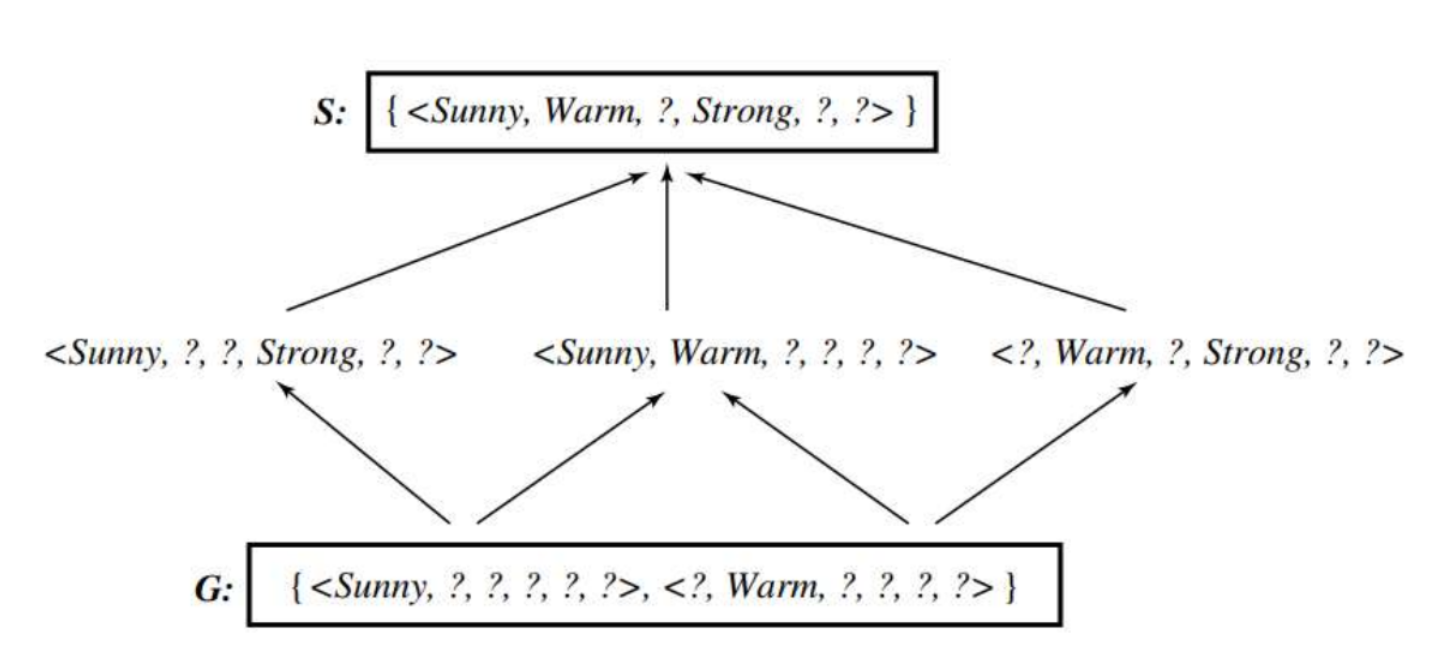
\includegraphics[width=1\linewidth]{images/finalbianxing.png}
        \caption{最终变形空间}
        \label{fig:placeholder}
    \end{figure}
    \item \textbf{一些论断：}
    \begin{itemize}
        \item 候选消除算法只有在训练数据无误且目标概念可由假设空间表示时，才能收敛到正确假设。
        \item 若训练数据存在错误，或目标概念不在假设空间中，则变型空间可能收敛为空集。
        \item 主动学习时，应优先选择能够将当前变型空间尽量二分的实例作为查询。
        \item 若变型空间中的所有假设对某实例给出相同分类，则该实例可被高置信度分类。
        \item 若不同假设对某实例给出不同分类，则该实例最能提供新的分类信息。
        \item 对未见实例的预测可由变型空间中的假设投票决定，票数比例可作为分类置信度。
    \end{itemize}
\end{enumerate}

\subsection{归纳偏置}\label{sec:inductive-bias}

\begin{enumerate}
    \item \textbf{归纳偏置的基本问题：}假设空间的表达能力不足。
    {\small\kaishu
    \begin{itemize}
        \item \textbf{问题：}Find-S和候选消除算法都假设目标概念一定在假设空间中，可是，当真如此吗？
        \item \textbf{解决办法：}为保证假设空间包含目标概念，一个直接办法是扩大假设空间，使每个可能的假设都被包含在内。
        \item \textbf{有偏的假设空间：}例如EnjoySport，仍把假设空间限制为只包含属性值的合取（“和”），则它不能表示简单的析取形式（“或”）目标概念，例如“Sky = Sunny 或 Sky = Cloudy”。在这种情况下，即使训练样例本身正确，算法也可能得到空的变型空间。原因在于：学习器偏向于只考虑合取式假设，这里需要表达能力更强的假设空间。
    \end{itemize}
    }
    \item \textbf{无偏学习器\footnote{觉得任何答案都一样可能，所以很难下结论。}与无偏学习的无用性：}归纳推理的一个基本属性：学习器如果不对目标概念的形式作预先假定，它从根本上无法对未见实例进行分类。
    {\small\kaishu
    \begin{itemize}
        \item 若要保证目标概念一定在假设空间中，就需要一个能够表达实例集 $X$ 的所有子集的假设空间，即 $X$ 的幂集。
        \item 这样虽然消除了表达能力不足的问题，却带来新的问题：概念学习算法将无法从训练样例中泛化。
    \end{itemize}
    }
    \item \textbf{归纳偏置的含义：}学习器能够从训练样例中泛化，原因就在于它带有归纳偏置，即假定目标概念可以由假设空间 $H$ 中的某个假设表示。
    {\small\kaishu
    \begin{itemize}
        \item 对候选消除算法而言，其归纳偏置可以写为
        \[
            \{\,c \in H\,\}
        \]
        \item 一般地，学习算法 $L$ 的归纳偏置是一个前提集合 $B$，使对任意新实例 $x_i$ 都有
        \[
            (B \land D_c \land x_i)\vdash L(x_i,D_c)
        \]
        \item 也就是说，学习器对新实例的分类，不仅依赖训练样例 $D_c$，还依赖于额外的前提集合 $B$ \footnote{学习器之所以敢对一个没见过的新样本$x_i$
下结论，不只是因为看过训练数据 $D$，还因为它偷偷额外相信了一些前提$B$}。
    \end{itemize}
    }
    \item \textbf{归纳偏置与归纳能力}
    \begin{itemize}
        \item 不同学习算法具有不同强度的归纳偏置（机械式、Find-S、候选消除算法）。
        \item 一种算法的有偏性越强，它的归纳能力越强，可以分类更多的未见实例\footnote{偏置越强，学习器越敢对没见过的样本下判断。}。
        \item 某些归纳偏置隐含在学习器中，有些则表示为断言集合，可由学习器操作。
    \end{itemize}
\end{enumerate}


\end{document}
